%% LyX 2.0.6 created this file.  For more info, see http://www.lyx.org/.
%% Do not edit unless you really know what you are doing.
\documentclass[twoside,english,british]{scrartcl}
\usepackage[T1]{fontenc}
\usepackage[latin9]{inputenc}
\usepackage{listings}
\usepackage{babel}
\usepackage{textcomp}
\usepackage{amsmath}
\usepackage[unicode=true,pdfusetitle,
 bookmarks=true,bookmarksnumbered=false,bookmarksopen=false,
 breaklinks=false,pdfborder={0 0 0},backref=false,colorlinks=false]
 {hyperref}

\makeatletter
%%%%%%%%%%%%%%%%%%%%%%%%%%%%%% Textclass specific LaTeX commands.
\numberwithin{equation}{section}
\numberwithin{figure}{section}
\numberwithin{table}{section}

%%%%%%%%%%%%%%%%%%%%%%%%%%%%%% User specified LaTeX commands.
\usepackage{graphicx}
\usepackage{listings}
\usepackage{color}
\usepackage{xcolor}
\usepackage{caption}
\usepackage{url}

  \usepackage{courier}
  \lstset{
  	basicstyle=\footnotesize\ttfamily, % Standardschrift
  	%numbers=left,               % Ort der Zeilennummern
  	numberstyle=\tiny,          % Stil der Zeilennummern
  	%stepnumber=2,               % Abstand zwischen den Zeilennummern
  	numbersep=5pt,              % Abstand der Nummern zum Text
  	tabsize=2,                  % Groesse von Tabs
  	extendedchars=true,         %
  	breaklines=true,            % Zeilen werden Umgebrochen
  	keywordstyle=\color{red},
  	frame=b,         
  	%        keywordstyle=[1]\textbf,    % Stil der Keywords
  	%        keywordstyle=[2]\textbf,    %
  	%        keywordstyle=[3]\textbf,    %
  	%        keywordstyle=[4]\textbf,   \sqrt{\sqrt{}} %
  	stringstyle=\color{white}\ttfamily, % Farbe der String
  	showspaces=false,           % Leerzeichen anzeigen ?
  	showtabs=false,             % Tabs anzeigen ?
  	xleftmargin=17pt,
  	framexleftmargin=17pt,
  	framexrightmargin=5pt,
  	framexbottommargin=4pt,
  	%backgroundcolor=\color{lightgray},
  	showstringspaces=false      % Leerzeichen in Strings anzeigen ?        
  }
  \lstloadlanguages{% Check Dokumentation for further languages ...
  	%[Visual]Basic
  	%Pascal
  	%C
  	%C++
  	%XML
  	%HTML
  	Java
  }
  %\DeclareCaptionFont{blue}{\color{blue}} 
  
  %\captionsetup[lstlisting]{singlelinecheck=false, labelfont={blue}, textfont={blue}}
  \usepackage{caption}
  
\DeclareCaptionFont{white}{\color{white}}
\DeclareCaptionFormat{listing}{\colorbox{gray}{\parbox{\textwidth}{#1#2#3}}}
\captionsetup[lstlisting]{format=listing,labelfont=white,textfont=white}

\makeatother

\begin{document}

\title{Internship Report}


\author{Philipp Glock}

\maketitle
\selectlanguage{english}%

\section{Introduction}

The division Federated Systems and Data of the Juelich Super Computing
Centre provides access to distributed resources like HPC systems and
data. This is done by implementing open standards and simplifying
usage and administration of these services. Therefor the division
is one of the core development partners of the UNICORE Grid middleware
and has members in the Research Data Alliance and the Open Grid Forum.

The research group High Productivity Data Processing works on solutions
to overcome problems and challenges occurring while handling 'big
data' problems. This can be splitted into three categories. 

\begin{enumerate} 	\item{\textbf{Investigate Generic Data Methods:}} How to overcome limitations of processing and analyzing large amounts of data ( e.g. in-memory databases, data privacy methods and query processing) 	\item{\textbf{Machine Learning:}} Use and extend serial or parallel machine learning techniques, like classification and clustering, to improve performance 	\item{\textbf{Smart Data Analytics Applications:}} Find and develop suitable applications for general data analysis 
\end{enumerate}

The goal of the internship is to build classification models for data
sets that show problems of 'big data' . Support Vector Machines are
the focused method, but other methods are considered as well. This
report shows the different problems and their solutions of several
approaches and implementations. \selectlanguage{british}%



\selectlanguage{english}%

\section{Background}

The primary programming language used during this internship is python.
Python is a dynamic scripting language and provides many nice modules
for scientific use cases like numpy and scipy. There are also some
machine learning modules and the scikit-learn module \cite{sklearn}
is one of the most used and stable ones. While python alone may not
have the best performance, it is easy to improve it by using c or
fortran code. This is done by most libraries. The serial support vector
machine algorithms of scikit-learn are based on the well known libsvm
library for example. This makes python and the scikit-learn module
a good choice for classification tasks. 

The tasks are executed on a super computer at the Juelich Supercomputing
Centre. It uses a PBS based batch system to handle the different jobs
of users and distribute the available nodes. A popular method for
distributed memory multiprocessing is MPI. It is, however, not being
used here.

IPython is an interactive python shell with many improvements. One
of them is interactive parallel computing. This allows parallelizing
python code in an interactive python session and has a robust error
handling. 

\lstinputlisting[language=bash,caption=pbs.controller.template,label=pbs_template]{./code/pbs.engine.template}

After setting up a profile and creating PBS templates (e.g. listing
\ref{pbs_template}), you can start a cluster easily using:

\[
ipcluster~start~--profile=pbs~-n~8
\]




More information on ipython in general and the setup for parallel
usage can be found at \cite{ipython_doc}.\selectlanguage{british}%


\section{Human Brain Project - brain analytics}


\subsection{The Project}

The Human Brain Project aims to acquire a better understanding of
the human brain by modeling it as a whole. One sub task of this project
is to build a 3d model of the human brain.

The brain analytics data set provides images of different cross sections
of a brain and each pixel is labeled whether it belongs to the cross
section or not. Labeling a whole brain takes a huge amount of time
and resources. So instead of labeling new images by hand, this data
is used to build a model that automatically classifies a pixel. If
this classification is good enough, the predicted 2d brain parts should
be used to rebuild a 3d model of a human brain. 

\begin{figure}[h] \centering \includegraphics[width=0.6\linewidth]{graphics/original603} \caption{An image of a cross section of a human brain} \label{fig:original603} \end{figure}

\section{Approach}


\subsection{The Data}

The data is not given as a classic table and therefor not directly
useable for classification. It consists of two sets of images. The
first one contains the original images of each cross section and a
corresponding mask. A mask is a grayscale image with only black or
white pixels. A pixel is white if it belongs to the cross section
and black if it does not. There are $762$ images with a resolution
of $3272\times2469$, resulting in a huge amount of pixels.

\begin{lstlisting}[caption=libsvm format,label=lisbsvm] 
<class_label> <feature_id>:value ... <feature_id>:value
<class_label> <feature_id>:value ... <feature_id>:value ... 
\end{lstlisting} 

The classification problem is a binary one since there are only two
classes. Before a classifier can be trained, the images have to be
converted into a attribute value format. The libsvm format was chosen,
because it is well known and many libraries support it. Every row
represents one instance, which is in this case one pixel and its features.
Currently the only features available are the rgb values of a pixel
from the original image and the class label from the mask. 


\subsection{Data Preparation}

In the first preprocessing step the libsvm data is created. The easiest
method saves for each pixel the rgb values and the class label. This
is done for every image resulting in $762$ files. Every file has
$8.078.568$ instances, so there are $6.155.868.816$ pixels in total.
A first trivial approach took about 3 days to generate all attribute
value files.

Building a model on this set would take a huge amount of time and
is therefor unreasonable for selecting a model. Instead of using the
complete data set samples have to be used. As figure \ref{fig:mask603}
shows there are more instances of class $0$ (black pixels) than of
class $1$ (white pixels). To weight both classes equally, the sampled
set is balanced. 

\begin{figure}	
\centering 	

\includegraphics[width=0.6\linewidth]{graphics/mask603} 	
\caption{Mask of a cross section} 	
\label{fig:mask603} 
\end{figure}

The first approach is a balanced random sampling method. For a given
percentage $p$ and a data set with \$N\$ instances the method draws
$p\cdot N$ samples from a file. If the sample is balanced, $p\cdot N\cdot0.5$
instances of each class are drawn randomly. This can easily be parallelized
since the files can be sampled independently. This yields a first
sample with three features. To improve the classifier the number of
features has to be increased.


\subsubsection{HSV color space}

An easy method to increase the number of features is to use another
color space in addition to the given RGB values. In this case the
HSV color space was chosen. It represents a color by its hue, saturation
and value. The values for a pixel can easily be transformed from RGB
to HSV with the following formula:

\begin{eqnarray*}
Max & = & max(R,G,B)\\
Min & = & min(R,G,B)\\
H & = & \begin{cases}
0, & \text{if Max =Min \ensuremath{\Leftrightarrow}}R=G=B\\
60\text{\textdegree}\cdot\left(0+\frac{G-B}{Max-Min}\right) & \text{if Max =R }\\
60\text{\textdegree}\cdot\left(2+\frac{B-R}{Max-Min}\right) & \text{if Max =G}\\
60\text{\textdegree}\cdot\left(4+\frac{R-G}{Max-Min}\right) & \text{if Max =B}
\end{cases}\\
S & = & \begin{cases}
0 & \text{if Max =0 \ensuremath{\Leftrightarrow}R=G=B=0 }\\
\frac{Max-Min}{Max} & else
\end{cases}\\
V & = & Max
\end{eqnarray*}


Since this computation can be done independently for every pixel,
the features can easily be computed in parallel and be added to existing
data. While computing the HSV values is simple, they also add only
few additional information. Because of this the increase of accuracy
is only marginal.

\begin{figure} 
\centering 
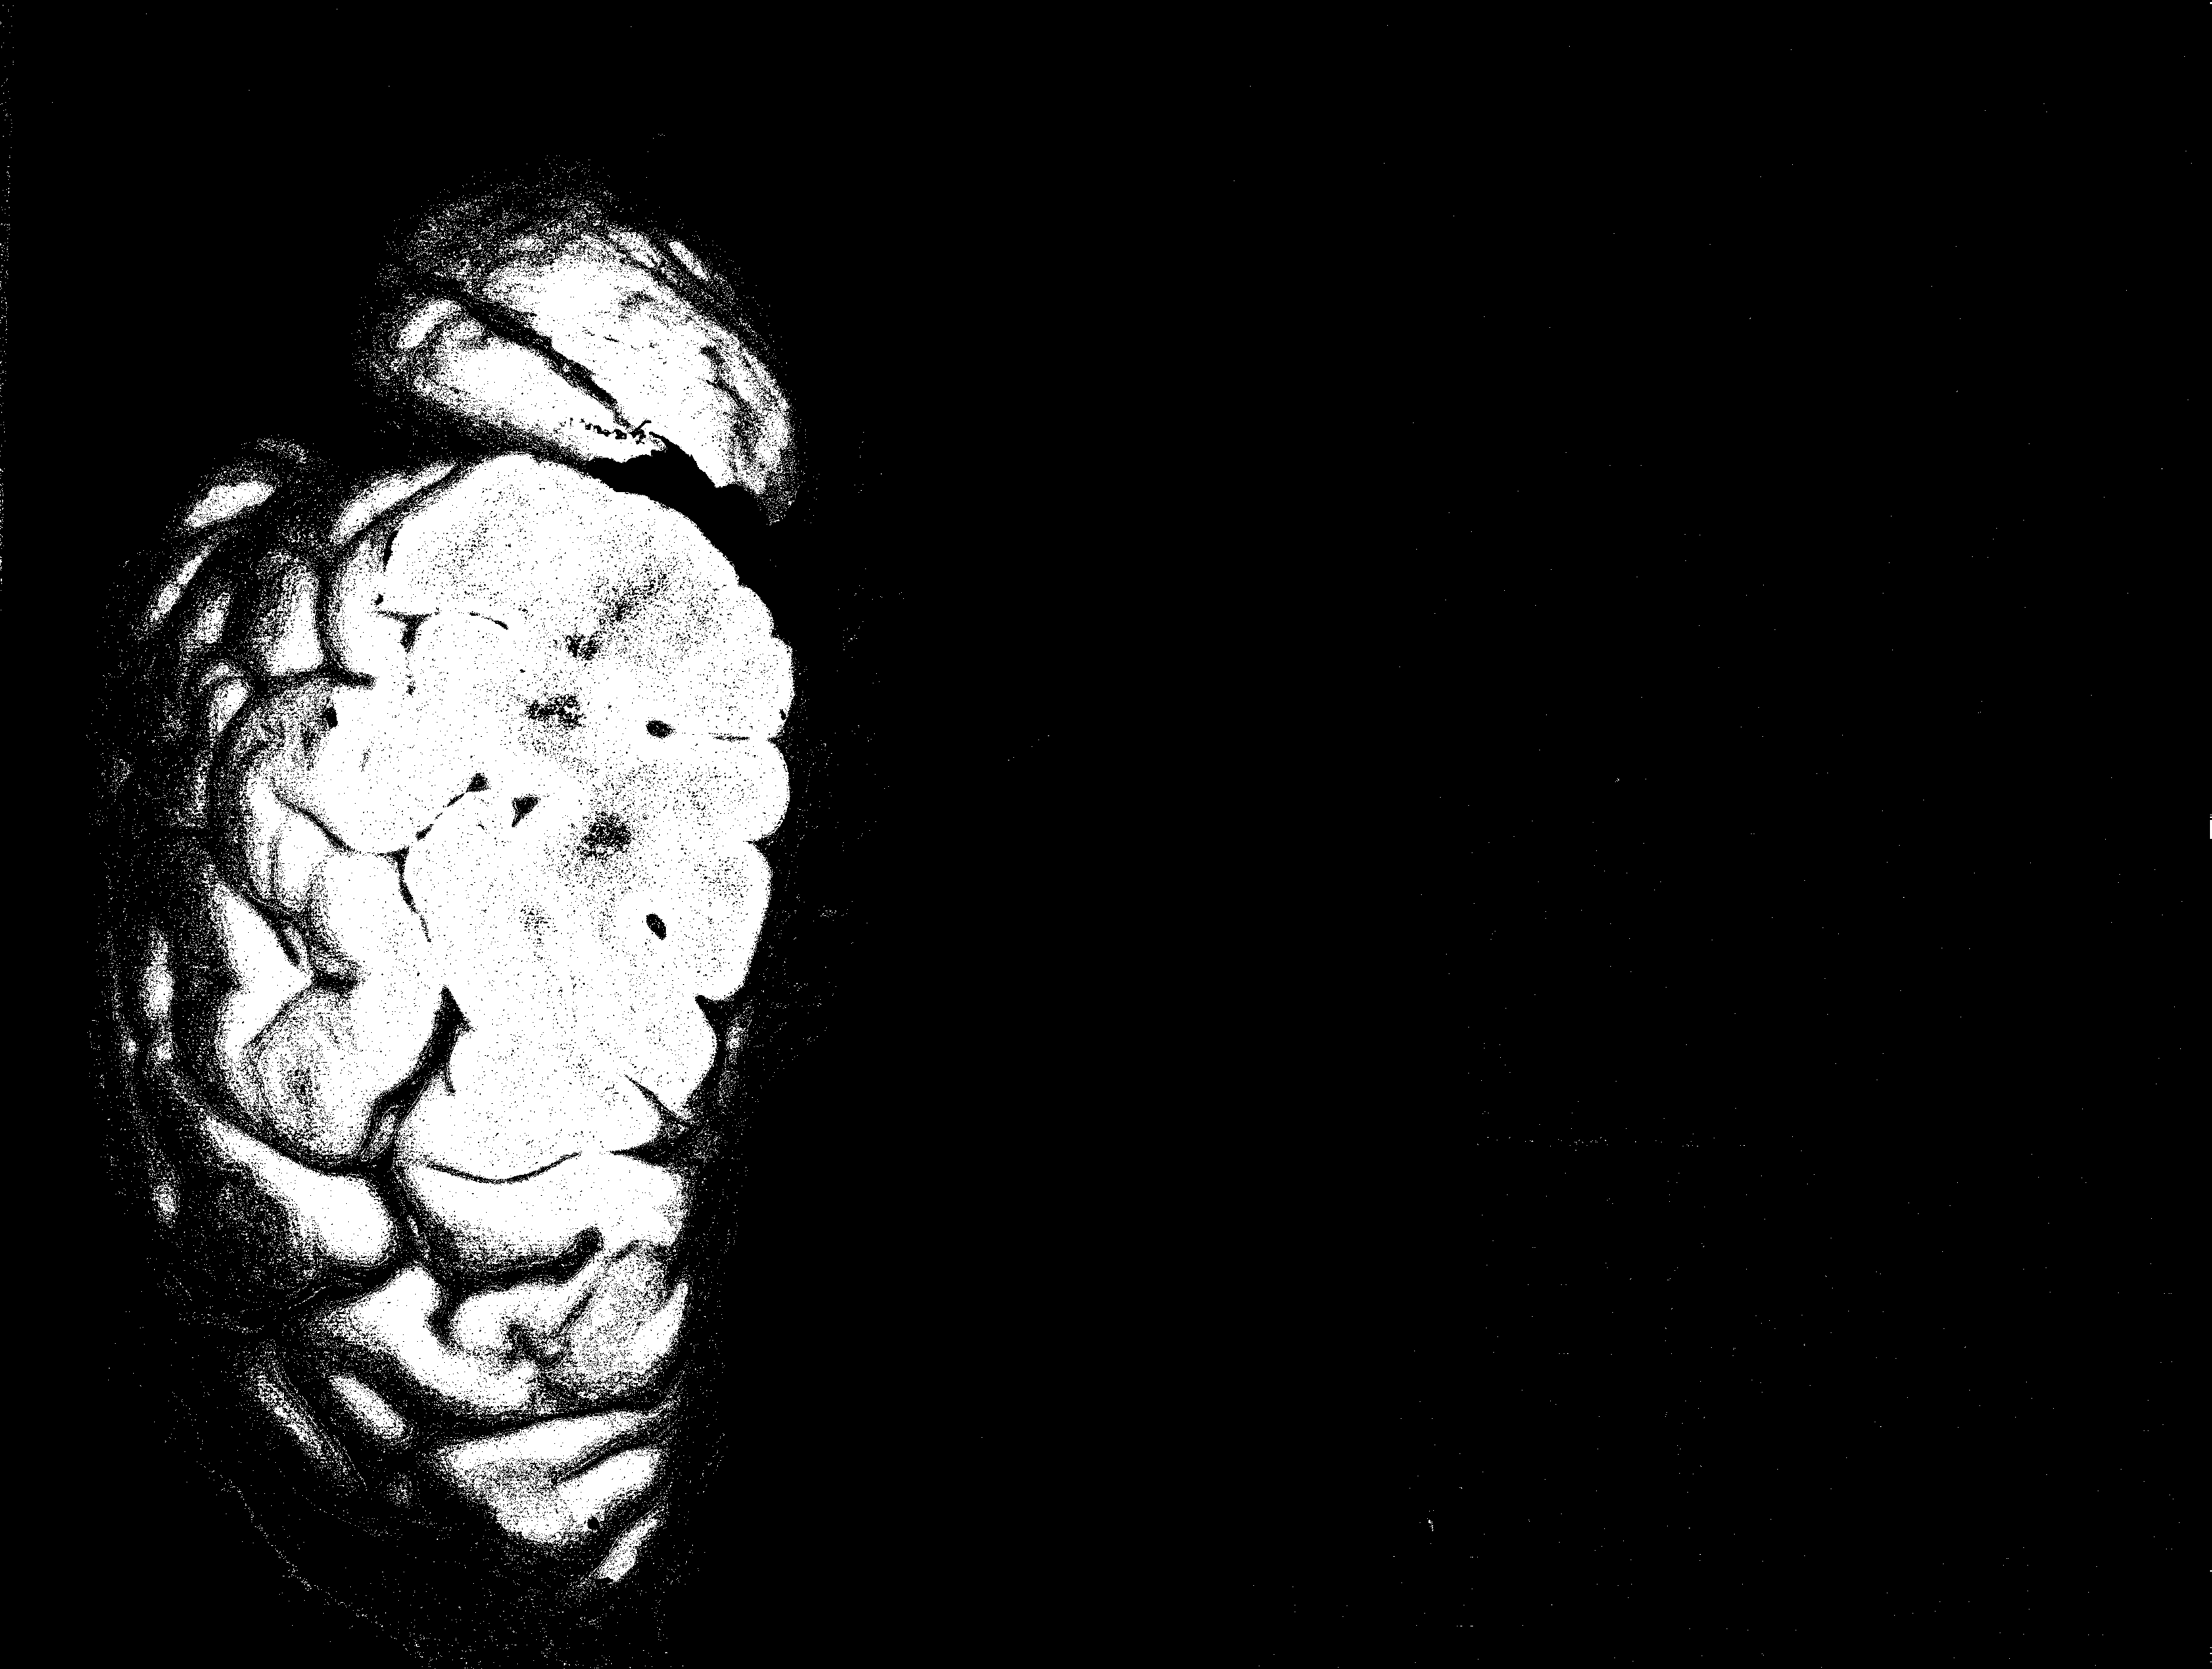
\includegraphics[width=0.7\linewidth]{graphics/predict200_svm_rbf} 
\caption{predicted image using svm with rbf kernel} 
\label{fig:predict200_svm_rbf} 
\end{figure}


\subsubsection{Local Features}

Despite adding the HSV color space, there is still no information
on the neighbourhood of a pixel. A first level approach to get information
on the neighbourhood of a pixel are statistical values like mean or
standard deviation. The statistical values are calculated on an $N\times N$
array around a pixel and assigned to the centered pixel. Figure \ref{calc_std}
shows how the standard deviation is calculated for an image. This
is done with the numpy and scipy modules. The \emph{generic\_filter}
function generates a window with the given size for every pixel and
calls the given function (e.g. numpy.std). 

\begin{figure}[H]


\begin{lstlisting}[language=Python,numbers=left]
def calc_std(img,size,use_mean=False):     
	"""Calculate the local standard deviation for each pixel of an image.
    Arguments:
        img : rgb image
        size : size of the window of neighbouring pixels
        use_mean : boolean, if False the standard deviation of R,G and B value are calculated and return as a 3 dimensional array.
                    if True the standard deviation of the mean is returned.
    Return:
      array_like, 3d or 2d
    """
    if not use_mean:
        std = np.zeros(img.shape)
        for i in range(img.shape[2]):
            std[:,:,i] = filters.generic_filter(img[:,:,i],np.std,size)
    else:
        mean_img = np.mean(img,axis=2)
        std = filters.generic_filter(mean_img,np.std,size)
    return std
\end{lstlisting}
\caption{Calculate the standard deviation using scipys generic\_filter method}
\label{calc_std}

\end{figure}



\subsubsection{Image Segmentation}


\subsection{Data Modeling}


\subsubsection{Support Vector Machines}

Support vector machines (SVMs) are one of the preferred classification
methods lately. They have a high accuracy, but their training time
is quite long. A model can easily be described by the found support
vectors.

SVMs can model nonlinear decision boundaries by using other kernels
instead of the linear kernel to increase the dimension of a vector.
A kernel defines the used scalar product. The most popular kernels
are the following:

\begin{itemize} 
\item linear:  $K(x,y) = \sum_{i=0}^n x_i\cdot y_i$ 
\item polynomial: $K(x,y) = (c+\sum_{i=0}^{n} x_i\cdot y_i)^d$	 	
\item rbf: $ \exp(-\frac{||x-y||^2}{2\sigma^2})$  
\end{itemize}  

\begin{figure}
\begin{tabular}{|l|r|r|r|}
\hline 	
Classifier 	& Accuracy & training time in s & test time in s \\  	
\hline 	
\hline 	
SVC (sklearn), rbf, 20k instances 	& 0.8752580408 	& 39.545465 	& 109.808209 	\\
\hline 	
\parbox[t]{6cm}{SVC (sklearn), rbf,\\ gamma=0.1, C=1, 20k instances} 	& 0.9579808675 	& 45.242423 	& 66.846724 \\  	
\hline 	
libSVM twister, 20k instances 	& 0.9592930497 	& 445.867 	& - \\  	
\hline 	
libSVM twister, 40k instances 	& 0.963317509 	& 934.912 	& - \\  	
\hline 	
libSVM twister, 100k instances 	& 0.9665214475 	& 3077.239 	& -\\ 	
\hline 
\end{tabular}  
\caption{SVMs from scikit-learn and Twister with rgb as features } 
\label{svm_table} 
\end{figure}

\begin{figure}
\begin{tabular}{|l|r|r|r|} 	
\hline 
Classifier & Accuracy & training time in s & test time in s \\  	
\hline 
GaussianNB & 0.9475908597 	& 0.042224 & 0.075098 \\  	
\hline 
Decision Tree & 0.9569552165 	& 0.563767 	& 0.057934 	\\  	
\hline 
RandomForest  & 0.9637635858 	& 1.698716 	& 0.399092 \\  	
\hline  
\end{tabular}  
\label{different_classifiers_table} 
\caption{Different classifiers used with rgb features.} 
\end{figure}

More information on SVMs can be found at \cite{Han2011}

\begin{figure} 
\centering 
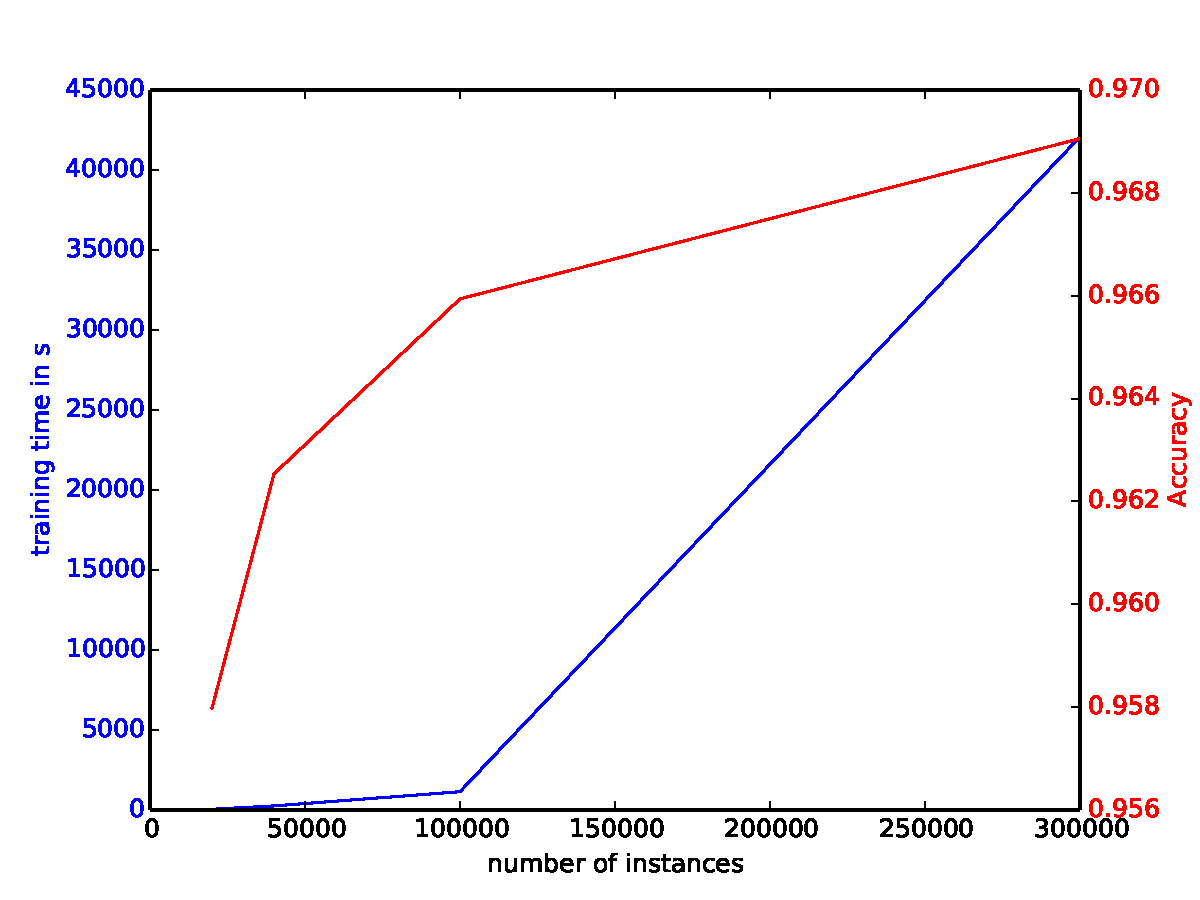
\includegraphics[width=0.8\linewidth]{graphics/sklearn_runtime} 
\caption{SVC training time with increasing sample} 
\label{fig:sklearn_runtime} 
\end{figure}


\subsection{Data Post Processing}


\subsection{Results}




\bibliographystyle{plain}
\phantomsection\addcontentsline{toc}{section}{\refname}\nocite{*}
\bibliography{refs}

\end{document}
